\documentclass[ openright,titlepage,numbers=noenddot,headinclude,%twoside,
                footinclude=true,BCOR=5mm,paper=a4,fontsize=11pt,a4paper,english%
                ]{scrreprt}
% ****************************************************************************************************
% classicthesis-config.tex 
% formerly known as loadpackages.sty, classicthesis-ldpkg.sty, and classicthesis-preamble.sty 
% Use it at the beginning of your ClassicThesis.tex, or as a LaTeX Preamble 
% in your ClassicThesis.{tex,lyx} with % ****************************************************************************************************
% classicthesis-config.tex 
% formerly known as loadpackages.sty, classicthesis-ldpkg.sty, and classicthesis-preamble.sty 
% Use it at the beginning of your ClassicThesis.tex, or as a LaTeX Preamble 
% in your ClassicThesis.{tex,lyx} with % ****************************************************************************************************
% classicthesis-config.tex 
% formerly known as loadpackages.sty, classicthesis-ldpkg.sty, and classicthesis-preamble.sty 
% Use it at the beginning of your ClassicThesis.tex, or as a LaTeX Preamble 
% in your ClassicThesis.{tex,lyx} with \input{classicthesis-config}
% ****************************************************************************************************  
% If you like the classicthesis, then I would appreciate a postca the postcards I received so far is available online at 
% http://postcards.miede.de
% ****************************************************************************************************

% ****************************************************************************************************
% 1. Configure classicthesis for your needs here, e.g., remove "drafting" below 
% in order to deactivate the time-stamp on the pages
% ****************************************************************************************************
\PassOptionsToPackage{eulerchapternumbers,listings,drafting,dottedtoc
				 pdfspacing,floatperchapter,linedheaders,
				 subfig,beramono,eulermath,parts}{classicthesis}										
% ********************************************************************
% Available options for classicthesis.sty 
% (see ClassicThesis.pdf for more information):
% drafting
% parts nochapters linedheaders
% eulerchapternumbers beramono eulermath pdfspacing minionprospacing
% tocaligned dottedtoc manychapters
% listings floatperchapter subfig
% ********************************************************************

% ********************************************************************
% Triggers for this config
% ******************************************************************** 
\usepackage{ifthen}
\newboolean{enable-backrefs} % enable backrefs in the bibliography
\setboolean{enable-backrefs}{false} % true false
% ****************************************************************************************************


% ****************************************************************************************************
% 2. Personal data and user ad-hoc commands
% ****************************************************************************************************
\newcommand{\myTitle}{A Classic Thesis Style\xspace}
\newcommand{\mySubtitle}{An Homage to The Elements of Typographic Style\xspace}
\newcommand{\myDegree}{Doktor-Ingenieur (Dr.-Ing.)\xspace}
\newcommand{\myName}{Andr\'e Miede\xspace}
\newcommand{\myProf}{Put name here\xspace}
\newcommand{\myOtherProf}{Put name here\xspace}
\newcommand{\mySupervisor}{Put name here\xspace}
\newcommand{\myFaculty}{Put data here\xspace}
\newcommand{\myDepartment}{Put data here\xspace}
\newcommand{\myUni}{Put data here\xspace}
\newcommand{\myLocation}{Darmstadt\xspace}
\newcommand{\myTime}{December 2011\xspace}
\newcommand{\myVersion}{version 4.0\xspace}

% ********************************************************************
% Setup, finetuning, and useful commands
% ********************************************************************
\newcounter{dummy} % necessary for correct hyperlinks (to index, bib, etc.)
\newlength{\abcd} % for ab..z string length calculation
\providecommand{\mLyX}{L\kern-.1667em\lower.25em\hbox{Y}\kern-.125emX\@}
\newcommand{\ie}{i.\,e.}
\newcommand{\Ie}{I.\,e.}
\newcommand{\eg}{e.\,g.}
\newcommand{\Eg}{E.\,g.} 
% ****************************************************************************************************


% ****************************************************************************************************
% 3. Loading some handy packages
% ****************************************************************************************************
% ******************************************************************** 
% Packages with options that might require adjustments
% ******************************************************************** 
\PassOptionsToPackage{utf8}{inputenc}	% latin9 (ISO-8859-9) = latin1+"Euro sign"
 \usepackage{inputenc}				

%\PassOptionsToPackage{ngerman,american}{babel}   % change this to your language(s)
% Spanish languages need extra options in order to work with this template
%\PassOptionsToPackage{spanish,es-lcroman}{babel}
 \usepackage{babel}					

\PassOptionsToPackage{square,numbers}{natbib}
 \usepackage{natbib}				

\PassOptionsToPackage{fleqn}{amsmath}		% math environments and more by the AMS 
 \usepackage{amsmath}

% ******************************************************************** 
% General useful packages
% ******************************************************************** 
\PassOptionsToPackage{T1}{fontenc} % T2A for cyrillics
	\usepackage{fontenc}                 
\usepackage{xspace} % to get the spacing after macros right  
\usepackage{mparhack} % get marginpar right
\usepackage{fixltx2e} % fixes some LaTeX stuff 
\PassOptionsToPackage{printonlyused,smaller}{acronym}
	\usepackage{acronym} % nice macros for handling all acronyms in the thesis
%\renewcommand*{\acsfont}[1]{\textssc{#1}} % for MinionPro
\renewcommand{\bflabel}[1]{{#1}\hfill} % fix the list of acronyms
% ****************************************************************************************************




% ****************************************************************************************************
% 4. Setup floats: tables, (sub)figures, and captions
% ****************************************************************************************************
\usepackage{tabularx} % better tables
	\setlength{\extrarowheight}{3pt} % increase table row height
\newcommand{\tableheadline}[1]{\multicolumn{1}{c}{\spacedlowsmallcaps{#1}}}
\newcommand{\myfloatalign}{\centering} % to be used with each float for alignment
\usepackage{caption}
\captionsetup{format=hang,font=small}
\usepackage{subfig}  
% ****************************************************************************************************


% ****************************************************************************************************
% 5. Setup code listings
% ****************************************************************************************************
\usepackage{listings} 
%\lstset{emph={trueIndex,root},emphstyle=\color{BlueViolet}}%\underbar} % for special keywords
\lstset{language=[LaTeX]Tex,%C++,
    keywordstyle=\color{RoyalBlue},%\bfseries,
    basicstyle=\small\ttfamily,
    %identifierstyle=\color{NavyBlue},
    commentstyle=\color{Green}\ttfamily,
    stringstyle=\rmfamily,
    numbers=none,%left,%
    numberstyle=\scriptsize,%\tiny
    stepnumber=5,
    numbersep=8pt,
    showstringspaces=false,
    breaklines=true,
    frameround=ftff,
    frame=single,
    belowcaptionskip=.75\baselineskip
    %frame=L
} 
% ****************************************************************************************************    		   


% ****************************************************************************************************
% 6. PDFLaTeX, hyperreferences and citation backreferences
% ****************************************************************************************************
% ********************************************************************
% Using PDFLaTeX
% ********************************************************************
\PassOptionsToPackage{pdftex,hyperfootnotes=false,pdfpagelabels}{hyperref}
	\usepackage{hyperref}  % backref linktocpage pagebackref
\pdfcompresslevel=9
\pdfadjustspacing=1 
\PassOptionsToPackage{pdftex}{graphicx}
	\usepackage{graphicx} 

% ********************************************************************
% Setup the style of the backrefs from the bibliography
% (translate the options to any language you use)
% ********************************************************************
\newcommand{\backrefnotcitedstring}{\relax}%(Not cited.)
\newcommand{\backrefcitedsinglestring}[1]{(Cited on page~#1.)}
\newcommand{\backrefcitedmultistring}[1]{(Cited on pages~#1.)}
\ifthenelse{\boolean{enable-backrefs}}%
{%
		\PassOptionsToPackage{hyperpageref}{backref}
		\usepackage{backref} % to be loaded after hyperref package 
		   \renewcommand{\backreftwosep}{ and~} % separate 2 pages
		   \renewcommand{\backreflastsep}{, and~} % separate last of longer list
		   \renewcommand*{\backref}[1]{}  % disable standard
		   \renewcommand*{\backrefalt}[4]{% detailed backref
		      \ifcase #1 %
		         \backrefnotcitedstring%
		      \or%
		         \backrefcitedsinglestring{#2}%
		      \else%
		         \backrefcitedmultistring{#2}%
		      \fi}%
}{\relax}    

% ********************************************************************
% Hyperreferences
% ********************************************************************
\hypersetup{%
    %draft,	% = no hyperlinking at all (useful in b/w printouts)
    colorlinks=true, linktocpage=true, pdfstartpage=3, pdfstartview=FitV,%
    % uncomment the following line if you want to have black links (e.g., for printing)
    %colorlinks=false, linktocpage=false, pdfborder={0 0 0}, pdfstartpage=3, pdfstartview=FitV,% 
    breaklinks=true, pdfpagemode=UseNone, pageanchor=true, pdfpagemode=UseOutlines,%
    plainpages=false, bookmarksnumbered, bookmarksopen=true, bookmarksopenlevel=1,%
    hypertexnames=true, pdfhighlight=/O,%nesting=true,%frenchlinks,%
    urlcolor=webbrown, linkcolor=RoyalBlue, citecolor=webgreen, %pagecolor=RoyalBlue,%
    %urlcolor=Black, linkcolor=Black, citecolor=Black, %pagecolor=Black,%
    pdftitle={\myTitle},%
    pdfauthor={\textcopyright\ \myName, \myUni, \myFaculty},%
    pdfsubject={},%
    pdfkeywords={},%
    pdfcreator={pdfLaTeX},%
    pdfproducer={LaTeX with hyperref and classicthesis}%
}   

% ********************************************************************
% Setup autoreferences
% ********************************************************************
% There are some issues regarding autorefnames
% http://www.ureader.de/msg/136221647.aspx
% http://www.tex.ac.uk/cgi-bin/texfaq2html?label=latexwords
% you have to redefine the makros for the 
% language you use, e.g., american, ngerman
% (as chosen when loading babel/AtBeginDocument)
% ********************************************************************
\makeatletter
\@ifpackageloaded{babel}%
    {%
       \addto\extrasamerican{%
					\renewcommand*{\figureautorefname}{Figure}%
					\renewcommand*{\tableautorefname}{Table}%
					\renewcommand*{\partautorefname}{Part}%
					\renewcommand*{\chapterautorefname}{Chapter}%
					\renewcommand*{\sectionautorefname}{Section}%
					\renewcommand*{\subsectionautorefname}{Section}%
					\renewcommand*{\subsubsectionautorefname}{Section}% 	
				}%
       \addto\extrasngerman{% 
					\renewcommand*{\paragraphautorefname}{Absatz}%
					\renewcommand*{\subparagraphautorefname}{Unterabsatz}%
					\renewcommand*{\footnoteautorefname}{Fu\"snote}%
					\renewcommand*{\FancyVerbLineautorefname}{Zeile}%
					\renewcommand*{\theoremautorefname}{Theorem}%
					\renewcommand*{\appendixautorefname}{Anhang}%
					\renewcommand*{\equationautorefname}{Gleichung}%        
					\renewcommand*{\itemautorefname}{Punkt}%
				}%
			% Fix to getting autorefs for subfigures right (thanks to Belinda Vogt for changing the definition)
			\providecommand{\subfigureautorefname}{\figureautorefname}%  			
    }{\relax}
\makeatother


% ****************************************************************************************************
% 7. Last calls before the bar closes
% ****************************************************************************************************
% ********************************************************************
% Development Stuff
% ********************************************************************
\listfiles
%\PassOptionsToPackage{l2tabu,orthodox,abort}{nag}
%	\usepackage{nag}
%\PassOptionsToPackage{warning, all}{onlyamsmath}
%	\usepackage{onlyamsmath}

% ********************************************************************
% Last, but not least...
% ********************************************************************
\usepackage{classicthesis} 

% Use arsclassica as well
\usepackage[dottedtoc]{arsclassica}
% ****************************************************************************************************


% ****************************************************************************************************
% 8. Further adjustments (experimental)
% ****************************************************************************************************
% ********************************************************************
% Changing the text area
% ********************************************************************
%\linespread{1.05} % a bit more for Palatino
%\areaset[current]{312pt}{761pt} % 686 (factor 2.2) + 33 head + 42 head \the\footskip
%\setlength{\marginparwidth}{7em}%
%\setlength{\marginparsep}{2em}%

% ********************************************************************
% Using different fonts
% ********************************************************************
%\usepackage[oldstylenums]{kpfonts} % oldstyle notextcomp
%\usepackage[osf]{libertine}
%\usepackage{hfoldsty} % Computer Modern with osf
%\usepackage[light,condensed,math]{iwona}
%\renewcommand{\sfdefault}{iwona}
%\usepackage{lmodern} % <-- no osf support :-(
%\usepackage[urw-garamond]{mathdesign} <-- no osf support :-(
% ****************************************************************************************************

% ****************************************************************************************************
% 9. Packages enabled by me
% ****************************************************************************************************
\usepackage{listings}
\usepackage{todonotes}
\usepackage{fancyhdr}
\usepackage[utf8]{fontenc}
\usepackage{babel}
\usepackage{booktabs}
\usepackage{cleveref}
\usepackage{setspace}
\usepackage{longtable}
\usepackage{needspace}

\usepackage[top=1.5in, bottom=1.2in, left=1in, right=1in]{geometry}

\usepackage{tikz}
\usetikzlibrary{shapes,arrows}
\usepackage{bigints}
\usetikzlibrary{shapes.geometric,shapes.arrows,arrows,backgrounds,fit,positioning,shapes.symbols,chains,decorations.pathmorphing}
%\usetikzlibrary{matrix,chains,scopes,positioning,arrows,fit}

\usepackage{amsmath, amssymb, amsthm}
\usepackage[T1]{fontenc}

% Set margins
%\addtolength{\oddsidemargin}{-.875in}
%\addtolength{\evensidemargin}{-.875in}
%\addtolength{\textwidth}{1.75in}

%\addtolength{\topmargin}{-.875in}
%\addtolength{\textheight}{1.75in}

% ****************************************************************************************************  
% If you like the classicthesis, then I would appreciate a postca the postcards I received so far is available online at 
% http://postcards.miede.de
% ****************************************************************************************************

% ****************************************************************************************************
% 1. Configure classicthesis for your needs here, e.g., remove "drafting" below 
% in order to deactivate the time-stamp on the pages
% ****************************************************************************************************
\PassOptionsToPackage{eulerchapternumbers,listings,drafting,dottedtoc
				 pdfspacing,floatperchapter,linedheaders,
				 subfig,beramono,eulermath,parts}{classicthesis}										
% ********************************************************************
% Available options for classicthesis.sty 
% (see ClassicThesis.pdf for more information):
% drafting
% parts nochapters linedheaders
% eulerchapternumbers beramono eulermath pdfspacing minionprospacing
% tocaligned dottedtoc manychapters
% listings floatperchapter subfig
% ********************************************************************

% ********************************************************************
% Triggers for this config
% ******************************************************************** 
\usepackage{ifthen}
\newboolean{enable-backrefs} % enable backrefs in the bibliography
\setboolean{enable-backrefs}{false} % true false
% ****************************************************************************************************


% ****************************************************************************************************
% 2. Personal data and user ad-hoc commands
% ****************************************************************************************************
\newcommand{\myTitle}{A Classic Thesis Style\xspace}
\newcommand{\mySubtitle}{An Homage to The Elements of Typographic Style\xspace}
\newcommand{\myDegree}{Doktor-Ingenieur (Dr.-Ing.)\xspace}
\newcommand{\myName}{Andr\'e Miede\xspace}
\newcommand{\myProf}{Put name here\xspace}
\newcommand{\myOtherProf}{Put name here\xspace}
\newcommand{\mySupervisor}{Put name here\xspace}
\newcommand{\myFaculty}{Put data here\xspace}
\newcommand{\myDepartment}{Put data here\xspace}
\newcommand{\myUni}{Put data here\xspace}
\newcommand{\myLocation}{Darmstadt\xspace}
\newcommand{\myTime}{December 2011\xspace}
\newcommand{\myVersion}{version 4.0\xspace}

% ********************************************************************
% Setup, finetuning, and useful commands
% ********************************************************************
\newcounter{dummy} % necessary for correct hyperlinks (to index, bib, etc.)
\newlength{\abcd} % for ab..z string length calculation
\providecommand{\mLyX}{L\kern-.1667em\lower.25em\hbox{Y}\kern-.125emX\@}
\newcommand{\ie}{i.\,e.}
\newcommand{\Ie}{I.\,e.}
\newcommand{\eg}{e.\,g.}
\newcommand{\Eg}{E.\,g.} 
% ****************************************************************************************************


% ****************************************************************************************************
% 3. Loading some handy packages
% ****************************************************************************************************
% ******************************************************************** 
% Packages with options that might require adjustments
% ******************************************************************** 
\PassOptionsToPackage{utf8}{inputenc}	% latin9 (ISO-8859-9) = latin1+"Euro sign"
 \usepackage{inputenc}				

%\PassOptionsToPackage{ngerman,american}{babel}   % change this to your language(s)
% Spanish languages need extra options in order to work with this template
%\PassOptionsToPackage{spanish,es-lcroman}{babel}
 \usepackage{babel}					

\PassOptionsToPackage{square,numbers}{natbib}
 \usepackage{natbib}				

\PassOptionsToPackage{fleqn}{amsmath}		% math environments and more by the AMS 
 \usepackage{amsmath}

% ******************************************************************** 
% General useful packages
% ******************************************************************** 
\PassOptionsToPackage{T1}{fontenc} % T2A for cyrillics
	\usepackage{fontenc}                 
\usepackage{xspace} % to get the spacing after macros right  
\usepackage{mparhack} % get marginpar right
\usepackage{fixltx2e} % fixes some LaTeX stuff 
\PassOptionsToPackage{printonlyused,smaller}{acronym}
	\usepackage{acronym} % nice macros for handling all acronyms in the thesis
%\renewcommand*{\acsfont}[1]{\textssc{#1}} % for MinionPro
\renewcommand{\bflabel}[1]{{#1}\hfill} % fix the list of acronyms
% ****************************************************************************************************




% ****************************************************************************************************
% 4. Setup floats: tables, (sub)figures, and captions
% ****************************************************************************************************
\usepackage{tabularx} % better tables
	\setlength{\extrarowheight}{3pt} % increase table row height
\newcommand{\tableheadline}[1]{\multicolumn{1}{c}{\spacedlowsmallcaps{#1}}}
\newcommand{\myfloatalign}{\centering} % to be used with each float for alignment
\usepackage{caption}
\captionsetup{format=hang,font=small}
\usepackage{subfig}  
% ****************************************************************************************************


% ****************************************************************************************************
% 5. Setup code listings
% ****************************************************************************************************
\usepackage{listings} 
%\lstset{emph={trueIndex,root},emphstyle=\color{BlueViolet}}%\underbar} % for special keywords
\lstset{language=[LaTeX]Tex,%C++,
    keywordstyle=\color{RoyalBlue},%\bfseries,
    basicstyle=\small\ttfamily,
    %identifierstyle=\color{NavyBlue},
    commentstyle=\color{Green}\ttfamily,
    stringstyle=\rmfamily,
    numbers=none,%left,%
    numberstyle=\scriptsize,%\tiny
    stepnumber=5,
    numbersep=8pt,
    showstringspaces=false,
    breaklines=true,
    frameround=ftff,
    frame=single,
    belowcaptionskip=.75\baselineskip
    %frame=L
} 
% ****************************************************************************************************    		   


% ****************************************************************************************************
% 6. PDFLaTeX, hyperreferences and citation backreferences
% ****************************************************************************************************
% ********************************************************************
% Using PDFLaTeX
% ********************************************************************
\PassOptionsToPackage{pdftex,hyperfootnotes=false,pdfpagelabels}{hyperref}
	\usepackage{hyperref}  % backref linktocpage pagebackref
\pdfcompresslevel=9
\pdfadjustspacing=1 
\PassOptionsToPackage{pdftex}{graphicx}
	\usepackage{graphicx} 

% ********************************************************************
% Setup the style of the backrefs from the bibliography
% (translate the options to any language you use)
% ********************************************************************
\newcommand{\backrefnotcitedstring}{\relax}%(Not cited.)
\newcommand{\backrefcitedsinglestring}[1]{(Cited on page~#1.)}
\newcommand{\backrefcitedmultistring}[1]{(Cited on pages~#1.)}
\ifthenelse{\boolean{enable-backrefs}}%
{%
		\PassOptionsToPackage{hyperpageref}{backref}
		\usepackage{backref} % to be loaded after hyperref package 
		   \renewcommand{\backreftwosep}{ and~} % separate 2 pages
		   \renewcommand{\backreflastsep}{, and~} % separate last of longer list
		   \renewcommand*{\backref}[1]{}  % disable standard
		   \renewcommand*{\backrefalt}[4]{% detailed backref
		      \ifcase #1 %
		         \backrefnotcitedstring%
		      \or%
		         \backrefcitedsinglestring{#2}%
		      \else%
		         \backrefcitedmultistring{#2}%
		      \fi}%
}{\relax}    

% ********************************************************************
% Hyperreferences
% ********************************************************************
\hypersetup{%
    %draft,	% = no hyperlinking at all (useful in b/w printouts)
    colorlinks=true, linktocpage=true, pdfstartpage=3, pdfstartview=FitV,%
    % uncomment the following line if you want to have black links (e.g., for printing)
    %colorlinks=false, linktocpage=false, pdfborder={0 0 0}, pdfstartpage=3, pdfstartview=FitV,% 
    breaklinks=true, pdfpagemode=UseNone, pageanchor=true, pdfpagemode=UseOutlines,%
    plainpages=false, bookmarksnumbered, bookmarksopen=true, bookmarksopenlevel=1,%
    hypertexnames=true, pdfhighlight=/O,%nesting=true,%frenchlinks,%
    urlcolor=webbrown, linkcolor=RoyalBlue, citecolor=webgreen, %pagecolor=RoyalBlue,%
    %urlcolor=Black, linkcolor=Black, citecolor=Black, %pagecolor=Black,%
    pdftitle={\myTitle},%
    pdfauthor={\textcopyright\ \myName, \myUni, \myFaculty},%
    pdfsubject={},%
    pdfkeywords={},%
    pdfcreator={pdfLaTeX},%
    pdfproducer={LaTeX with hyperref and classicthesis}%
}   

% ********************************************************************
% Setup autoreferences
% ********************************************************************
% There are some issues regarding autorefnames
% http://www.ureader.de/msg/136221647.aspx
% http://www.tex.ac.uk/cgi-bin/texfaq2html?label=latexwords
% you have to redefine the makros for the 
% language you use, e.g., american, ngerman
% (as chosen when loading babel/AtBeginDocument)
% ********************************************************************
\makeatletter
\@ifpackageloaded{babel}%
    {%
       \addto\extrasamerican{%
					\renewcommand*{\figureautorefname}{Figure}%
					\renewcommand*{\tableautorefname}{Table}%
					\renewcommand*{\partautorefname}{Part}%
					\renewcommand*{\chapterautorefname}{Chapter}%
					\renewcommand*{\sectionautorefname}{Section}%
					\renewcommand*{\subsectionautorefname}{Section}%
					\renewcommand*{\subsubsectionautorefname}{Section}% 	
				}%
       \addto\extrasngerman{% 
					\renewcommand*{\paragraphautorefname}{Absatz}%
					\renewcommand*{\subparagraphautorefname}{Unterabsatz}%
					\renewcommand*{\footnoteautorefname}{Fu\"snote}%
					\renewcommand*{\FancyVerbLineautorefname}{Zeile}%
					\renewcommand*{\theoremautorefname}{Theorem}%
					\renewcommand*{\appendixautorefname}{Anhang}%
					\renewcommand*{\equationautorefname}{Gleichung}%        
					\renewcommand*{\itemautorefname}{Punkt}%
				}%
			% Fix to getting autorefs for subfigures right (thanks to Belinda Vogt for changing the definition)
			\providecommand{\subfigureautorefname}{\figureautorefname}%  			
    }{\relax}
\makeatother


% ****************************************************************************************************
% 7. Last calls before the bar closes
% ****************************************************************************************************
% ********************************************************************
% Development Stuff
% ********************************************************************
\listfiles
%\PassOptionsToPackage{l2tabu,orthodox,abort}{nag}
%	\usepackage{nag}
%\PassOptionsToPackage{warning, all}{onlyamsmath}
%	\usepackage{onlyamsmath}

% ********************************************************************
% Last, but not least...
% ********************************************************************
\usepackage{classicthesis} 

% Use arsclassica as well
\usepackage[dottedtoc]{arsclassica}
% ****************************************************************************************************


% ****************************************************************************************************
% 8. Further adjustments (experimental)
% ****************************************************************************************************
% ********************************************************************
% Changing the text area
% ********************************************************************
%\linespread{1.05} % a bit more for Palatino
%\areaset[current]{312pt}{761pt} % 686 (factor 2.2) + 33 head + 42 head \the\footskip
%\setlength{\marginparwidth}{7em}%
%\setlength{\marginparsep}{2em}%

% ********************************************************************
% Using different fonts
% ********************************************************************
%\usepackage[oldstylenums]{kpfonts} % oldstyle notextcomp
%\usepackage[osf]{libertine}
%\usepackage{hfoldsty} % Computer Modern with osf
%\usepackage[light,condensed,math]{iwona}
%\renewcommand{\sfdefault}{iwona}
%\usepackage{lmodern} % <-- no osf support :-(
%\usepackage[urw-garamond]{mathdesign} <-- no osf support :-(
% ****************************************************************************************************

% ****************************************************************************************************
% 9. Packages enabled by me
% ****************************************************************************************************
\usepackage{listings}
\usepackage{todonotes}
\usepackage{fancyhdr}
\usepackage[utf8]{fontenc}
\usepackage{babel}
\usepackage{booktabs}
\usepackage{cleveref}
\usepackage{setspace}
\usepackage{longtable}
\usepackage{needspace}

\usepackage[top=1.5in, bottom=1.2in, left=1in, right=1in]{geometry}

\usepackage{tikz}
\usetikzlibrary{shapes,arrows}
\usepackage{bigints}
\usetikzlibrary{shapes.geometric,shapes.arrows,arrows,backgrounds,fit,positioning,shapes.symbols,chains,decorations.pathmorphing}
%\usetikzlibrary{matrix,chains,scopes,positioning,arrows,fit}

\usepackage{amsmath, amssymb, amsthm}
\usepackage[T1]{fontenc}

% Set margins
%\addtolength{\oddsidemargin}{-.875in}
%\addtolength{\evensidemargin}{-.875in}
%\addtolength{\textwidth}{1.75in}

%\addtolength{\topmargin}{-.875in}
%\addtolength{\textheight}{1.75in}

% ****************************************************************************************************  
% If you like the classicthesis, then I would appreciate a postca the postcards I received so far is available online at 
% http://postcards.miede.de
% ****************************************************************************************************

% ****************************************************************************************************
% 1. Configure classicthesis for your needs here, e.g., remove "drafting" below 
% in order to deactivate the time-stamp on the pages
% ****************************************************************************************************
\PassOptionsToPackage{eulerchapternumbers,listings,drafting,dottedtoc
				 pdfspacing,floatperchapter,linedheaders,
				 subfig,beramono,eulermath,parts}{classicthesis}										
% ********************************************************************
% Available options for classicthesis.sty 
% (see ClassicThesis.pdf for more information):
% drafting
% parts nochapters linedheaders
% eulerchapternumbers beramono eulermath pdfspacing minionprospacing
% tocaligned dottedtoc manychapters
% listings floatperchapter subfig
% ********************************************************************

% ********************************************************************
% Triggers for this config
% ******************************************************************** 
\usepackage{ifthen}
\newboolean{enable-backrefs} % enable backrefs in the bibliography
\setboolean{enable-backrefs}{false} % true false
% ****************************************************************************************************


% ****************************************************************************************************
% 2. Personal data and user ad-hoc commands
% ****************************************************************************************************
\newcommand{\myTitle}{A Classic Thesis Style\xspace}
\newcommand{\mySubtitle}{An Homage to The Elements of Typographic Style\xspace}
\newcommand{\myDegree}{Doktor-Ingenieur (Dr.-Ing.)\xspace}
\newcommand{\myName}{Andr\'e Miede\xspace}
\newcommand{\myProf}{Put name here\xspace}
\newcommand{\myOtherProf}{Put name here\xspace}
\newcommand{\mySupervisor}{Put name here\xspace}
\newcommand{\myFaculty}{Put data here\xspace}
\newcommand{\myDepartment}{Put data here\xspace}
\newcommand{\myUni}{Put data here\xspace}
\newcommand{\myLocation}{Darmstadt\xspace}
\newcommand{\myTime}{December 2011\xspace}
\newcommand{\myVersion}{version 4.0\xspace}

% ********************************************************************
% Setup, finetuning, and useful commands
% ********************************************************************
\newcounter{dummy} % necessary for correct hyperlinks (to index, bib, etc.)
\newlength{\abcd} % for ab..z string length calculation
\providecommand{\mLyX}{L\kern-.1667em\lower.25em\hbox{Y}\kern-.125emX\@}
\newcommand{\ie}{i.\,e.}
\newcommand{\Ie}{I.\,e.}
\newcommand{\eg}{e.\,g.}
\newcommand{\Eg}{E.\,g.} 
% ****************************************************************************************************


% ****************************************************************************************************
% 3. Loading some handy packages
% ****************************************************************************************************
% ******************************************************************** 
% Packages with options that might require adjustments
% ******************************************************************** 
\PassOptionsToPackage{utf8}{inputenc}	% latin9 (ISO-8859-9) = latin1+"Euro sign"
 \usepackage{inputenc}				

%\PassOptionsToPackage{ngerman,american}{babel}   % change this to your language(s)
% Spanish languages need extra options in order to work with this template
%\PassOptionsToPackage{spanish,es-lcroman}{babel}
 \usepackage{babel}					

\PassOptionsToPackage{square,numbers}{natbib}
 \usepackage{natbib}				

\PassOptionsToPackage{fleqn}{amsmath}		% math environments and more by the AMS 
 \usepackage{amsmath}

% ******************************************************************** 
% General useful packages
% ******************************************************************** 
\PassOptionsToPackage{T1}{fontenc} % T2A for cyrillics
	\usepackage{fontenc}                 
\usepackage{xspace} % to get the spacing after macros right  
\usepackage{mparhack} % get marginpar right
\usepackage{fixltx2e} % fixes some LaTeX stuff 
\PassOptionsToPackage{printonlyused,smaller}{acronym}
	\usepackage{acronym} % nice macros for handling all acronyms in the thesis
%\renewcommand*{\acsfont}[1]{\textssc{#1}} % for MinionPro
\renewcommand{\bflabel}[1]{{#1}\hfill} % fix the list of acronyms
% ****************************************************************************************************




% ****************************************************************************************************
% 4. Setup floats: tables, (sub)figures, and captions
% ****************************************************************************************************
\usepackage{tabularx} % better tables
	\setlength{\extrarowheight}{3pt} % increase table row height
\newcommand{\tableheadline}[1]{\multicolumn{1}{c}{\spacedlowsmallcaps{#1}}}
\newcommand{\myfloatalign}{\centering} % to be used with each float for alignment
\usepackage{caption}
\captionsetup{format=hang,font=small}
\usepackage{subfig}  
% ****************************************************************************************************


% ****************************************************************************************************
% 5. Setup code listings
% ****************************************************************************************************
\usepackage{listings} 
%\lstset{emph={trueIndex,root},emphstyle=\color{BlueViolet}}%\underbar} % for special keywords
\lstset{language=[LaTeX]Tex,%C++,
    keywordstyle=\color{RoyalBlue},%\bfseries,
    basicstyle=\small\ttfamily,
    %identifierstyle=\color{NavyBlue},
    commentstyle=\color{Green}\ttfamily,
    stringstyle=\rmfamily,
    numbers=none,%left,%
    numberstyle=\scriptsize,%\tiny
    stepnumber=5,
    numbersep=8pt,
    showstringspaces=false,
    breaklines=true,
    frameround=ftff,
    frame=single,
    belowcaptionskip=.75\baselineskip
    %frame=L
} 
% ****************************************************************************************************    		   


% ****************************************************************************************************
% 6. PDFLaTeX, hyperreferences and citation backreferences
% ****************************************************************************************************
% ********************************************************************
% Using PDFLaTeX
% ********************************************************************
\PassOptionsToPackage{pdftex,hyperfootnotes=false,pdfpagelabels}{hyperref}
	\usepackage{hyperref}  % backref linktocpage pagebackref
\pdfcompresslevel=9
\pdfadjustspacing=1 
\PassOptionsToPackage{pdftex}{graphicx}
	\usepackage{graphicx} 

% ********************************************************************
% Setup the style of the backrefs from the bibliography
% (translate the options to any language you use)
% ********************************************************************
\newcommand{\backrefnotcitedstring}{\relax}%(Not cited.)
\newcommand{\backrefcitedsinglestring}[1]{(Cited on page~#1.)}
\newcommand{\backrefcitedmultistring}[1]{(Cited on pages~#1.)}
\ifthenelse{\boolean{enable-backrefs}}%
{%
		\PassOptionsToPackage{hyperpageref}{backref}
		\usepackage{backref} % to be loaded after hyperref package 
		   \renewcommand{\backreftwosep}{ and~} % separate 2 pages
		   \renewcommand{\backreflastsep}{, and~} % separate last of longer list
		   \renewcommand*{\backref}[1]{}  % disable standard
		   \renewcommand*{\backrefalt}[4]{% detailed backref
		      \ifcase #1 %
		         \backrefnotcitedstring%
		      \or%
		         \backrefcitedsinglestring{#2}%
		      \else%
		         \backrefcitedmultistring{#2}%
		      \fi}%
}{\relax}    

% ********************************************************************
% Hyperreferences
% ********************************************************************
\hypersetup{%
    %draft,	% = no hyperlinking at all (useful in b/w printouts)
    colorlinks=true, linktocpage=true, pdfstartpage=3, pdfstartview=FitV,%
    % uncomment the following line if you want to have black links (e.g., for printing)
    %colorlinks=false, linktocpage=false, pdfborder={0 0 0}, pdfstartpage=3, pdfstartview=FitV,% 
    breaklinks=true, pdfpagemode=UseNone, pageanchor=true, pdfpagemode=UseOutlines,%
    plainpages=false, bookmarksnumbered, bookmarksopen=true, bookmarksopenlevel=1,%
    hypertexnames=true, pdfhighlight=/O,%nesting=true,%frenchlinks,%
    urlcolor=webbrown, linkcolor=RoyalBlue, citecolor=webgreen, %pagecolor=RoyalBlue,%
    %urlcolor=Black, linkcolor=Black, citecolor=Black, %pagecolor=Black,%
    pdftitle={\myTitle},%
    pdfauthor={\textcopyright\ \myName, \myUni, \myFaculty},%
    pdfsubject={},%
    pdfkeywords={},%
    pdfcreator={pdfLaTeX},%
    pdfproducer={LaTeX with hyperref and classicthesis}%
}   

% ********************************************************************
% Setup autoreferences
% ********************************************************************
% There are some issues regarding autorefnames
% http://www.ureader.de/msg/136221647.aspx
% http://www.tex.ac.uk/cgi-bin/texfaq2html?label=latexwords
% you have to redefine the makros for the 
% language you use, e.g., american, ngerman
% (as chosen when loading babel/AtBeginDocument)
% ********************************************************************
\makeatletter
\@ifpackageloaded{babel}%
    {%
       \addto\extrasamerican{%
					\renewcommand*{\figureautorefname}{Figure}%
					\renewcommand*{\tableautorefname}{Table}%
					\renewcommand*{\partautorefname}{Part}%
					\renewcommand*{\chapterautorefname}{Chapter}%
					\renewcommand*{\sectionautorefname}{Section}%
					\renewcommand*{\subsectionautorefname}{Section}%
					\renewcommand*{\subsubsectionautorefname}{Section}% 	
				}%
       \addto\extrasngerman{% 
					\renewcommand*{\paragraphautorefname}{Absatz}%
					\renewcommand*{\subparagraphautorefname}{Unterabsatz}%
					\renewcommand*{\footnoteautorefname}{Fu\"snote}%
					\renewcommand*{\FancyVerbLineautorefname}{Zeile}%
					\renewcommand*{\theoremautorefname}{Theorem}%
					\renewcommand*{\appendixautorefname}{Anhang}%
					\renewcommand*{\equationautorefname}{Gleichung}%        
					\renewcommand*{\itemautorefname}{Punkt}%
				}%
			% Fix to getting autorefs for subfigures right (thanks to Belinda Vogt for changing the definition)
			\providecommand{\subfigureautorefname}{\figureautorefname}%  			
    }{\relax}
\makeatother


% ****************************************************************************************************
% 7. Last calls before the bar closes
% ****************************************************************************************************
% ********************************************************************
% Development Stuff
% ********************************************************************
\listfiles
%\PassOptionsToPackage{l2tabu,orthodox,abort}{nag}
%	\usepackage{nag}
%\PassOptionsToPackage{warning, all}{onlyamsmath}
%	\usepackage{onlyamsmath}

% ********************************************************************
% Last, but not least...
% ********************************************************************
\usepackage{classicthesis} 

% Use arsclassica as well
\usepackage[dottedtoc]{arsclassica}
% ****************************************************************************************************


% ****************************************************************************************************
% 8. Further adjustments (experimental)
% ****************************************************************************************************
% ********************************************************************
% Changing the text area
% ********************************************************************
%\linespread{1.05} % a bit more for Palatino
%\areaset[current]{312pt}{761pt} % 686 (factor 2.2) + 33 head + 42 head \the\footskip
%\setlength{\marginparwidth}{7em}%
%\setlength{\marginparsep}{2em}%

% ********************************************************************
% Using different fonts
% ********************************************************************
%\usepackage[oldstylenums]{kpfonts} % oldstyle notextcomp
%\usepackage[osf]{libertine}
%\usepackage{hfoldsty} % Computer Modern with osf
%\usepackage[light,condensed,math]{iwona}
%\renewcommand{\sfdefault}{iwona}
%\usepackage{lmodern} % <-- no osf support :-(
%\usepackage[urw-garamond]{mathdesign} <-- no osf support :-(
% ****************************************************************************************************

% ****************************************************************************************************
% 9. Packages enabled by me
% ****************************************************************************************************
\usepackage{listings}
\usepackage{todonotes}
\usepackage{fancyhdr}
\usepackage[utf8]{fontenc}
\usepackage{babel}
\usepackage{booktabs}
\usepackage{cleveref}
\usepackage{setspace}
\usepackage{longtable}
\usepackage{needspace}

\usepackage[top=1.5in, bottom=1.2in, left=1in, right=1in]{geometry}

\usepackage{tikz}
\usetikzlibrary{shapes,arrows}
\usepackage{bigints}
\usetikzlibrary{shapes.geometric,shapes.arrows,arrows,backgrounds,fit,positioning,shapes.symbols,chains,decorations.pathmorphing}
%\usetikzlibrary{matrix,chains,scopes,positioning,arrows,fit}

\usepackage{amsmath, amssymb, amsthm}
\usepackage[T1]{fontenc}

% Set margins
%\addtolength{\oddsidemargin}{-.875in}
%\addtolength{\evensidemargin}{-.875in}
%\addtolength{\textwidth}{1.75in}

%\addtolength{\topmargin}{-.875in}
%\addtolength{\textheight}{1.75in}


\begin{document}

\title{
\Large{\textbf{Eugene: Agent-Based Market Simulator for use in Validation and System Testing of Trading Algorithms}}\\[1.2cm]
\normalsize{Jakub Koz\l{}owski \\
Internal Supervisor: Dr. Christopher D. Clack \\
External Supervisor: Ian Rose-Miller, UBS \\[1.2cm]
Department of Computer Science \\University College London \\[1cm]}
\small{April 2011}
}
\author{} \date{}

\maketitle
\tableofcontents
\chapter*{Abstract}
At 3:40 PM on November 14\textsuperscript{th}, 2007, a buggy Credit Suisse proprietary algorithm (SmartWB) sent approximately 600,000 cancel/replace messages for non existent orders, triggerring 450,000 error messages from the NYSE and leading to a disruption of trading, with 131,000 messages frozen in queue that could not be processed and ultimately had to be deleted. Credit Suisse was fined \$150,000.~\cite{Nyse2009} On May 6, 2010, U.S. stock market has experienced a sudden price drop of 5\%, followed by a rapid recovery, in the mean time sending Accenture share price to a single cent and Sotheby’s to \$99,999.99, all in the course of about 30 minutes. Subsequent analyses of the incident concluded that the the incident was triggered by a large sell program that lead to "hot-potato" effect, where in the 14-second period more than 27,000 futures contracts were bought and sold, with the net effect of only around 200 contracts.~\cite{Kirilenko2011}

These prominent examples of software errors in Trading Algorithms highlight an urgent issue with the way these systems are tested. In order to prevent Trading Algorithms from exhibiting such behaviour, there is a need for a strategy of rigorous testing in a realistic environment. Current testing techniques (backtesting on historical data) fail to capture the dynamic nature of markets and hence may fail to identify flaws in the Trading Algorithms. In this thesis we demonstrate an Agent-Based Stock Market Simulator and evaluate its efficacy in automatic discovery of software errors in Trading Algorithms.
\vfill

\pagestyle{scrheadings}

\chapter{Introduction}
\label{Chapters/Introduction}
\section{Motivation}
The design of a software system gradually evolves over time, as the understanding of the problem domain improves and the business requirements change. The cost of change of a software system is not negligible, however it is relatively low in comparison to other Engineering Disciplines \marginpar{I need to see if I can find a reference to back this up}and can be controlled by adhering to principles of good design and by following software development processes~\cite{Gof1995}. This propensity encourages iterative approach to software development; controlled improvements, extensions and revisions of the artefacts move the system from one version to the next(Agile). 

The key to controlled evolution of a software system is to rely on rigorous testing and validation at all levels of the architecture: from testing individual units of code (Unit Testing), through testing interfaces between components (Integration Testing), to testing a completely integrated software system (System Testing). Recent trends in software development practices even encourage the tests of a functionality to be written prior to the sourcecode~\cite{Beck2001}. It is argued that such systems tend to have low-coupling, as their design needs to accommodate testing components in isolation and control over the dependencies, however evidence is contradictory as to the exact effects of following this practice~\cite{Siniaalto2007}.

In order to ensure the correct operation of a software system over time, all the levels of testing need to be automatic and fast, in order to encourage the developers to perform them locally, following every change (Automated Testing, Continuous Integration). Adhering to those principles reduces reliance on manual testing, prevents regression errors in existing functionality (Regression Testing) and improves release time.

These principles apply well to deterministic systems; testing comes down to verifying that a set of inputs will produce a particular set of outputs, because the operation of such a system can be approximated with a deterministic-state machine. The difficulty occurs when dealing with non-deterministic systems; testing involves verifying that a particular set of inputs will produce a correct set of outputs with a statistically significant probability.

Since mid-80s, financial markets have been undergoing a phase of extensive automation of the way order flows are handled. First revolution took place with the introduction of electronic markets with an open access to the limit order book, that replaced traditional, open-outcry markets. However, since mid-2000s, a second revolution is in the making: Trading Algorithms have been replacing human traders in the process of negotiating prices and reducing market impact. Those sophisticated real-time systems, designed to replicate certain trading patterns, have a clear advantage over human traders in the amount of information they can take into account, as well as the speed at which they are able to take positions~\cite{Lenglet}.

The actions of the Trading Algorithms take an active part in shaping the market dynamics and, although constantly monitored, they sometimes contribute to \emph{flash crashes}: brief periods of extreme market volatility. On May 6, 2010, U.S. stock market has experienced a sudden price drop of 5\%, followed by a rapid recovery, all in the course of about 30 minutes. One subsequent analysis of that incident concluded that:
\begin{quote}
[$\ldots$] technological innovation is critical for market development. However, as markets change, appropriate safeguards must be implemented to keep pace with trading practices enabled by advances in technology~\cite{Kirilenko2011}.
\end{quote}
Overall, lack of rigorous testing of Trading Algorithms and other trading systems does not only affect the P\&L  of the owner of the technology, but may also lead to systemic instability of the market.

Trading Algorithms are an example of a non-deterministic system that operates in a highly non-deterministic environment. They are designed to respond to the situation on the market and to have a certain expectation as to the effect their actions will have on the market.

Traditionally, \marginpar{'Traditionally' is probably not the best word}Trading Algorithms are backtested on historical data by rebuilding the past order flows on the limit order book. Certain characteristics can be measured (e.g. VWAP of the algorithm) and compared to corresponding benchmarks (e.g. VWAP of the Market) to evaluate whether the algorithm is doing the right thing. This approach can give certain level of confidence as to the correct operation of the trading algorithm, however it nonetheless fails to model the reactions of other market participants to the order flows coming from the algorithm~\cite{Coggins2006}.

In recent years, the Agent-Based Modelling (ABM) approach has been applied to understanding the complex phenomena observed in economic and financial systems. An Agent-Based Model is a computer simulation of evolving and autonomous software decision makers (agents) that interact through a set of prescribed rules. Applying ABM models to financial markets offers possibility of studying how behaviour of individual agents affects the overall market dynamics~\citep{Sorban2008, Farmer2009}. Most widely discussed approaches to Agent-Based Artificial Stock Markets implement discrete time, call markets and employ various techniques in order to simulate traders' behaviour~\cite{Jha2010}.

In an attempt to supplement the strategy of backtesting Trading Algorithms on historical data and address its shortcomings, in this report we propose \emph{Eugene}: a real-time, continuous trading session Agent-Based Artificial Stock Market for Validation and System Testing of Trading Algorithms. We aim to demonstrate that simulations involving simple market participants (Noise Traders) can be used for discovering a class of logical polarity programming errors and differentiating between Trading Algorithms.

We will start by formulating the research objectives and null-hypotheses, followed by a discussion of the research methodologies.





\section{Research Objective and Null Hypotheses}
\section{Research methodology}
\section{Outline of the Report \label{Chapters/Introduction/Outline}}

In \Cref{Chapters/Background/Market-Microstructure} we describe the model of the market mechanism we will use in the simulator. We describe the market architectures employed in the stock exchanges during continuous trading sessions, namely model of limit order book, and how it enables market participants to interact asynchronously.

In \Cref{Chapters/Background/Agent-Based-Modelling} we summarise several artificial stock markets from the available literature. We provide a model of zero-intelligence agents that will be implemented by the Noise Traders, that is based on the work by~\citet[chap.~4]{Gilles2006}. Moreover, in order to provide a background for implementing a VWAP Trading Algorithm for the experiments, we survey available sources, most prominently the work in~\cite{Coggins2006, Kakade2004}. 

\Cref{Chapters/Analysis-and-Design} and \ref{Chapters/Implementation} provide a summary of the main requirements that informed the design and highlight main principles that guided the implementation of the simulator. We describe main elements of an Algorithmic Trading System and \textit{Eugene's} place in that architecture. We provide the pseudo code for the algorithms implemented for the Noise Traders and VWAP Traders.

\Cref{Chapters/Testing-and-Validation} summarises the steps taken to evaluate the implementation of the simulation, as well as it's efficacy in Testing Trading Algorithms. The results and analysis of experiments described in \Cref{Chapters/Implementation} are presented. Different levels of testing as they apply to the simulator are explained, from \textit{Unit-Testing} to following the method employed in~\cite[chap.~4]{Gilles2006} in order to validate the implementation of the Noise Traders.

Finally, in \Cref{Chapters/Conclusion-and-Further-Work} we summarise the key points of this work, highlight the testing method developed and its applicability to testing Trading Algorithms. We then review the contributions and achievements and then provide the possible extensions on how to take this work forward.





\chapter{Background}
\label{Chapters/Background}
\section{The limit order book market architecture}
\label{Chapters/Background/Market-Architecture}

In this section we describe the model of the market mechanism we will use in the simulator. We describe the market architectures employed in the stock exchanges during continuous trading sessions, namely model of limit order book, and how it enables market participants to interact asynchronously. 

\subsection{}

\section{Agent-Based Artificial Stock Markets}
\label{Chapters/Background/Agent-Based-Modelling}

In this section we summarise several artificial stock markets from the available literature. We provide a model of zero-intelligence agents that will be implemented by the Noise Traders, that is based on the work by~\citet[chap.~4]{Gilles2006}. Moreover, in order to provide a background material for implementing a VWAP Trading Algorithm for the experiments, we survey available sources, most prominently the work in~\cite{Coggins2006, Kakade2004}. 

\subsection{Agent-Based Modelling}
Agent-Based Modelling is a simulation technique concerned with designing societies of rule-based software agents that interact in particular ways, with a view of assessing the of of individual (or groups of) agents on the system as a whole. This technique has been successfully applied in many business scenarios, including financial simulations. Among the benefits of agent-based modelling is emergent phenomena: behaviour resulting from complex interactions of many individual entities.

\subsection{Agent-Based Computational Economics}
Agent-Based Models that attempt to explain economic processes are branded as Agent-Based Computational Economics. In recent years, studying stock markets using multi-agent based models has become a promising research area due to the fact that this methodology reflects the fundamental nature of a stock market, where the current situation is a result of a complex interaction of actions of many heterogenous investors that have various expectations and different levels of rationality.

\subsection{An overview of Agent-Based Artificial Stock Markets}

\subsubsection*{SantaFe ASM~\citep{Lebaron2002, Lebaron99}}
The Santa Fe Artificial Stock Market is a discrete time Artificial Stock Market that consists a central computational market and a number of intelligent agent. Agents make decision by attempting to forecast the future returns on the stock using genetic programming and therefore decide between investing in stock or leaving their money in the bank, which pays a fixed interest rate.

The simulated market consists of $N$ agents, usually $50-100$, that interact with the market. The stock has the price $p(t)$ per share at time $t$, where $p(t)$ is set endogenously to clear the market (\textit{call market}). The stock pays a dividend $d(t+1)$ at the end of time $t$, according to a stochastic process, independent of the market and agents' actions. The money left in the bank pays constant rate of return of $r$ per period. The information available to agents consists of the price, the dividend, total number of bids/asks at each past period, plus some additional variables. 

By using genetic programming, agents can explore a wide range of possible forecasting rules and they have the flexibility to use or disregard certain pieces of avaiable information. The market was able to generate the key stylised facts: weak forecastability, volatility persistence, and higher expected returns.~\cite{Lebaron99}. 

\subsubsection{Genoa ASM~\citep{}}










\chapter{Analysis and Design}
\label{Chapters/Analysis-and-Design}
\section{Trading System Design}

%\begin{figure}[H]
%\centerline{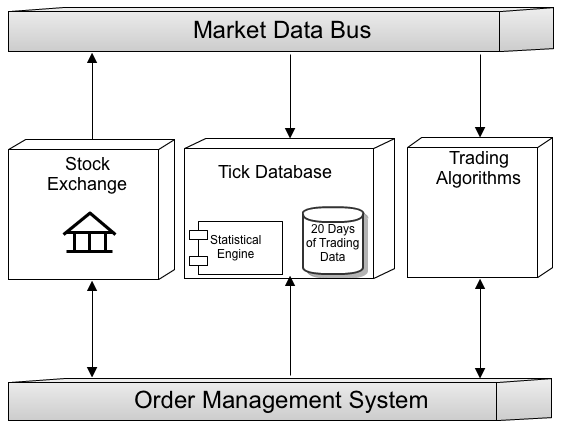
\includegraphics[scale=0.6]{trading-system-design.png}}
%\caption{Trading System Architecture}
%\label{fig:trading-system-architecture}
%\end{figure}

\subsection{Stock Exchange}
Market Participants submit orders to the Stock Exchange in order to trade. Stock Exchanges publish messages about the submitted/executed orders.

\subsection{Market Data Bus}
Market Data Bus subscribes to messages published by different Stock Exchanges in order to publish them in a standardised way to various internal systems, e.g. Trading Algorithms.

\subsection{Order Management System}
Registers with various Stock Exchanges in order to provide a standardised way of submitting orders by various internal systems, e.g. Trading Algorithms, and also allow Automatic Order Routing between different Stock Exchanges.

\subsection{Tick Database}
Subscribes to the Market Data Bus in order to perform a statistical analysis on the behaviour of different stocks. The result of the statistical analysis is a set of parameters which describe various aspects of stock behaviour. The parameters are published to various internal systems, e.g. Trading Algorithms.

\subsection{Trading Algorithms}
Highly sophisticated and parameterised systems which accept orders and execute them using different strategies. Trading Algorithms register with the Market Data Bus in order to react to the current situation on the market. They continuously compare the behaviour of stocks with their historical behaviour (using data from the Tick Database) in order to quickly discover unexpected behaviour. 

\section{Automated Trading Algorithm Testing Environment}

\begin{figure}[H]
\centerline{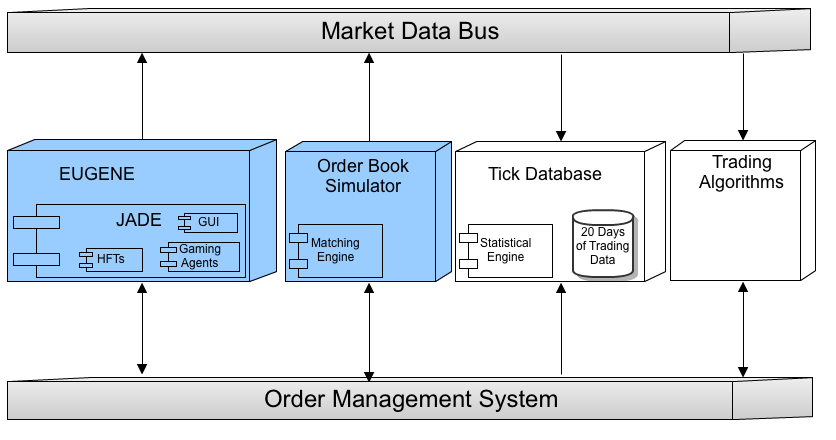
\includegraphics[scale=0.5]{architectural-description/automated-trading-testing-environment.png}}
\caption{Automated Trading Algorithm Testing Environment}
\label{fig:automated-trading-algorithm-testing-environment}
\end{figure}

Trading Algorithms respond to messages received from the Stock Exchange (via the Market Data Bus) and send orders to the Stock Exchange (via the Order Management System). They expect the orders to have some influence on the situation on the Stock Exchange. 

Therefore, in order to setup a testing environment for Trading Algorithms, two systems need to be put in place in order to simulate the Trading System.

\subsection{Order Book Simulator}
Order Matching Engine which can accept orders in to Continuous Auction Trading and match Bid/Sell orders. The simulator should be programmable to handle any number of exchanges and stocks. Such an engine is already available for use and will not be the subject of this project.

\subsection{Market Behaviour Simulator}
Market Behaviour Simulator that can realistically simulate a broad range of market behaviours (e.g. rising and falling, flash crash, gaming). This project will propose a design of such a Market Simulator using an Agent-Based Approach.

\section{Eugene: Agent-Based Market Simulator}

\subsection{Approach}
Agent-Based simulation is a powerful technique that has been successfully applied in many business scenarios, including financial simulations. Among the benefits of agent-based modelling is emergent phenomena: behaviour resulting from complex interactions of many individual entities. 

Therefore, whereas in a real stock market, the current situation is a result of a complex interaction of many market players, it is hypothesised that an interaction of several types of software agents will result in an emergence of realistic market behaviour.

\subsection{Technologies}
\subsubsection{Java Agent DEvelopment Framework}
\texttt{JADE} is a software framework for developing distributed, multi-agent software systems in Java. \texttt{JADE} can be deployed onto a set of containers (nodes) which together form a platform (cluster).

Each platform has a \texttt{Main Container} which holds two special agents:
\begin{itemize}
\item The \texttt{Agent Management System} (AMS) which can create and kill agents, kill containers and shut down the entire platform.
\item The \texttt{Directory Facilitator} (DF) which implements a \texttt{yellow pages} service.
\end{itemize} 

Each agent in \texttt{JADE} operates in a separate thread of control, therefore allowing independent, preemptive behaviour. \texttt{JADE}  has been designed to operate within an \texttt{OSGi} container, therefore making it easier to deploy.

\subsubsection{Open Services Gateway initiative framework}
\texttt{OSGi} is dynamic module and service system platform for Java. Application components (distributed as \texttt{bundles}) can be remotely managed without requiring a reboot of the entire container. A package management system enables developers to package public and private APIs within the same bundle, but only expose public APIs at runtime. The dynamic service system allows the components to discover the addition of new services and act accordingly.

\subsection{Simulation Structure}
\begin{itemize} 
\item Eugene will simulate one day of a continuous auction trading.
\item Eugene will aim to simulate a set of typical markets, according to parameters such as: Volume Curve, Price Volatility, Bid/Ask spread, average order size etc. (list not exhaustive).
\item Eugene will aim to simulate the following set of agents (list is not exhaustive):
\begin{itemize}
\item High Frequency Trading Agent: agent that moves in and out of short-term positions many times each day, to capture trading opportunities that may open up only for fractions of a second.
\item Gaming Agent: agent that is designed to try to trick Trading Algorithms in order to manipulate them for its own gain.
\item Random Agent: agent that will make random decisions to send mid, aggressive or passive orders.
\item Technical Analysis Agent: agent that will make decisions based on past behaviour of the market.
\item etc.
\end{itemize}
\end{itemize}

\subsection{Aims}
\begin{itemize}
\item Analyse existing Agent-Based approaches to Market Simulation to determine a set of possible Agent Types.
\item Implement the Agents.
\item Discover a specific configuration of Agents whose behaviour will simulate each target market, in regards to a set of pre-determined market characteristics (Volume Curve, Price Volatility etc.).
\item Analyse efficacy of the Agent-Based Market Simulation approach for use in System Testing of Trading Algorithms.
\end{itemize}

\subsection{Success Factors}
\begin{itemize}
\item Develop a realistic simulation for at least one target market.
\end{itemize}


\chapter{Implementation}
\label{implementation}

\section{Things to draw attention to}
\begin{itemize}
\item The principle of defensive programming.
\item Separation of concerns with extensive use of programming to an interface.
\item Information hiding with use of private packages (OSGi) that contain implementations;
\item Hiding implementations behind factories.
\item Modularised design.
\item Extensive unit and integration testing.
\item jade-unit.
\item mocking.
\item Careful consideration of threading issues and hence multithreaded design.

\end{itemize}


\chapter{Testing and Validation}
\label{testing}

\chapter{Conclusion and Further Work}
\label{conclusion}

%\end{onehalfspace}

%\begin{singlespace}
%\begin{footnotesize}
%\begin{twocolumn}
\bibliographystyle{IEEEtran}
\bibliography{Bibliography}
%\end{twocolumn}
%\end{footnotesize}
%\end{singlespace}

\end{document}
